\documentclass{llncs}

\usepackage{ifpdf}
\ifpdf
  \usepackage[pdftex]{graphicx}
  \graphicspath{{./pdf/}{./jpeg/}{./eps/}}
  \DeclareGraphicsExtensions{.pdf,.jpeg,.png}
\else
  \usepackage[dvips]{graphicx}
  \graphicspath{{./eps/}}
  \DeclareGraphicsExtensions{.eps}
\fi

\usepackage[cmex10]{amsmath}
\usepackage{amsfonts}
\usepackage[noend]{algpseudocode}
\usepackage{algorithm}
\algnewcommand{\LineComment}[1]{\State \(\triangleright\) #1}
\usepackage[tight,footnotesize]{subfigure}
\begin{document}

\title{Bisection and Twisted Bidiagonal SVD on GPU for Big Matrices}

\author{Lu He\inst{1}, Yan Luo\inst{1}, Rui Liu\inst{1}, Hengyong Yu\inst{1}, Yu Cao\inst{1}, Xuzhou Chen\inst{3} and Seung Woo Son\inst{1}}

\institute{University of Massachusetts Lowell, Lowell MA 01854, USA
\and
Fitchburg State University, Fitchburg MA 01420, USA}

\maketitle
\input{0_abstract}
%\begin{abstract}
%The abstract should summarize the contents of the paper
%using at least 70 and at most 150 words. It will be set in 9-point
%font size and be inset 1.0 cm from the right and left margins.
%There will be two blank lines before and after the Abstract. \dots
%\end{abstract}
%

\section{Introduction}
\label{sec:intro}
There is rapidly growing interest in singular value decomposition (SVD) in various fields,
including noise reduction in signal processing,
low-rank approximations in linear algebra, 
objects classification in computer vision,
latent semantic indexing in information retrieval,
supervised and unsupervised algorithms in machine learning,
and data compression in information theory.
Yet, most algorithms for computing SVD are designed to solve problems
with only small-scale data in acceptable time and space requirements
due to their algorithmic complexities.
With the advent of the ``big data'' era, these algorithms are no longer adequate in terms of computational complexity and required memory space.

A typical SVD algorithm can be broken down into two steps\cite{65SIAM}.
The first step is to reduce the initial matrix to bidiagonal form using Householder transformation.
The second step is to diagonalize the resulting matrix using bidiagonal SVD algorithms.
Most of the literature focuses on the second step as algorithms in second step typically use iterative approaches\cite{58iter1,90iter2,65iter3} and thus take majority of the computation time depending on the accuracy requirement.

There are many algorithms for solving the bidiagonal SVD. 
QR iteration is regarded as a powerful and effective approach
%, and yet the fastest algorithm 
for finding all the singular values.
%However, it is only the fastest algorithm for matrices of size 25 or smaller\cite{97bookalgebra}.
Due to its complexity of $O(n^3)$, QR's execution time increases rapidly as the size of a matrix increases.
Jacobi algorithm is the one with the highest accuracy in practice\cite{97bookalgebra}.
However, its $O(n^3)$ complexity with a big constant causes the algorithm to be much slower than other algorithms, making the iteration times much larger than those of QR algorithm.

Divide-and-conquer (DC) is assumed to be the fastest algorithm for finding singular values for large matrices\cite{94DCSVD}.
It takes $O(n^{2.3})$ flops on average\cite{97bookalgebra}. 
In the worst case, it may require up to $O(n^3)$.
But the major drawback of DC is the relatively low accuracy of the
singular values when merging, let alone singular vectors. 
In summary, the prior works on SVD computations are either time-consuming or inaccurate.

In addition, all the algorithms discussed above have two common disadvantages:
%\begin{enumerate}
%\item 
(1) heavy data dependence makes SVD algorithm not suitable for parallelization and extension for other architectures; and
(2) large memory space required for temporary variables
%The large memory space needed for these algorithms will 
dramatically limits the capability for computing singular values for very large matrices.
%\end{enumerate}

Many SVD applications, such as principal component
analysis (PCA), need only a small subset of the singular values and
vectors. However, the aforementioned algorithms lack the flexibility of calculating the subsets directly.
Bisection and inverse (BI) iteration method could calculate the subset of the singular values and vectors\cite{95ETNAbisecion} as well as the complete SVD.
In this method, bisection is responsible for obtaining singular
values, while inverse iteration is responsible for singular vectors
with obtained singular values.
BI takes $O(kn)$ to find $k$ singular values and singular vectors. 
%and $O(k^2n)$ in the worst case of $k$ singular values are clustered\cite{97bookalgebra}.
%It is much faster than other algorithms especially when only a small subset of singular values and vectors are needed for large matrices.
However, the inverse iteration does not guarantee the accuracy and orthogonality of the computed singular vectors in the case of clustered singular values.
%\textcolor{blue}{
%Fortunately, twisted algorithm is able to calculate the accurate and orthogonal singular vectors\cite{09NLAAtwisted}.
%}

In this paper, we present a new SVD approach called ``Bisection and Twisted'' (BT) algorithm. We use the twisted algorithm \cite{09NLAAtwisted} to replace the inverse iteration in BI, because the twisted algorithm is able to calculate accurate and orthogonal singular vectors. 
%The BT algorithm inherits the advantages of both Bisection and twisted algorithms\cite{09NLAAtwisted}.
Comparing to other algorithms, BT approach only requires $O(n^2)$ to complete the whole SVD\cite{09NLAAtwisted,05UCB}, and $O(kn)$ to calculate $k$ singular values and corresponding vectors.
Most importantly, there are three salient features that make BT algorithm attractive
to obtaining SVD of large matrices. First, the data dependency is weak in the BT algorithm because it does not need to synchronize intermediate results for the following calculation (as in other algorithms),
making it an excellent candidate for taking advantage of the parallel computing
elements (e.g., multicore CPUs or GPUs). Second, 
the algorithm can obtain a subset of $k$ singular values and its corresponding vectors in $O(kn)$ time. This is particularly useful for applications that
do not require a complete SVD.
Third, the algorithm needs only $O(kn)$ memory space to store
temporary variables, which is important for extending to large scale
matrices in big data applications on memory constrained platforms.

We then design GPU kernels to implement the BT algorithm on GPU platforms. We evaluate its performance on a variety of GPUs to study its scalability. 
We also design a multi-GPU version of BT to demonstrate 
the effectiveness of weak data dependency and scale it
to compute the SVD of very large matrices. We are able to solve
SVD of a matrix of 1 million by 1 million using only two GPUs. 

In this paper, we make the following contributions:
\begin{enumerate}
\item We propose a novel SVD algorithm called Bisection and Twisted for fast SVD computation. It requires $O(n^2)$ time to solve the complete SVD, and $O(kn)$
for calculating a subset of $k$ singular vectors.
\item We show that the data dependency of BT algorithm is weak.
As a result, BT algorithm is highly suitable for massively parallel computing architecture on which we can effectively partition a large problem into smaller ones.
\item We not only implement the BT algorithm on different GPUs, but also design a multi-GPU version that can scale well with the matrix size. To the best of our knowledge, we are the first to achieve SVD on a one million by one million matrix using just two GPUs.
\item We perform in-depth analysis on the GPU kernels for singular vector calculation, and present multiple optimization methods to further improve the SVD performance on GPUs.
\end{enumerate}

The rest of the paper is organized as follows.
The Bisection and Twisted algorithm is given in Section \ref{sec:algorithm}.
Section \ref{sec:implementation} describes the implementation of the BT algorithm on GPUs, as well as the GPU specific optimizations.
Section \ref{sec:results} presents the experimental results and profiling analysis of GPU kernels.
Section \ref{sec:related} discusses the related work.
Conclusion and future work are in Section \ref{sec:conclusion}.



\vspace{-0.1in}
\section{Bisection and Twisted Algorithm} \label{sec:algorithm}
\vspace{-0.1in}
For an arbitrary matrix $A\in \mathbb{R}^{m \times n} (m>n)$, 
A SVD of an arbitrary matrix $A\in \mathbb{R}^{m \times n} (m>n)$ is the form $A = U \Sigma V^T$, where $U$ is a $m \times m$ orthogonal matrix, $V$ is a $n\times n$ orthogonal matrix, and $\Sigma$ is a $m\times n$ diagonal matrix.
A typical SVD algorithm can be broken down into two steps \cite{65SIAM}.
The first step is to reduce the initial matrix to bidiagonal by Householder transform.
The second step is to diagonalize the bidiagonal matrix.
Householder transform above has been optimized in paper \cite{LiuHouseholder} for small matrices. For very large matrices, it is still an open problem. 
In this paper, we focus only on the second step that reduces a bidiagonal matrix to a diagonal matrix, for which the  ``bisection and twisted'' algorithm is designed.

%\begin{equation}
%A = Q B P^T
%\label{eq:householder}
%\end{equation}
%where $B \in \mathbb{R}^{m \times n}$ is a bidiagonal matrix of the form $ B = ( B_1, 0 )^T$.
%Here $B_1 \in \mathbb{R}^{n \times n}$ is a bidiagonal matrix. 
%Since $B^T B = (B_1^T, 0)(B_1, 0)^T = B_1^T B_1$,
%we assume, without loss of generality, that $B$ is a $n \times n$ bidiagonal matrix in this paper.
 
The bisection and twisted algorithm is divided into two phases:
(1) obtain the singular values of the bidiagonal matrix by bisection approach; and
(2) obtain the corresponding left and right singular vectors of every singular value by twisted factorization.
Next we describe these two phases in the following subsections.

\vspace{-0.1in}
\subsection{Bisection Algorithm}\label{subsec:bisection}
\vspace{-0.1in}
Suppose $B$ is an upper bidiagonal $n \times n$ matrix with elements $b_{i,j}$ reduced by Householder transform \cite{10householder}.
The matrix $T = B^T B - \mu^2 I_n$ can be decomposed as
\begin{equation}
\label{eq:T}
T = B^T B - \mu^2 I_n = L D L^T ,
\end{equation}
where $\mu$ is a shift variable, $D=diag(d_1,d_2,\cdots,d_n)$ and $L$ is lower bidiagonal matrix, whose diagonal elements are $1$s and one-order subdiagonal elements are $l_{i}, (i=1,\cdots,n-1)$.
%are as below.
%\[ D =  \left( \begin{array}{cccc}
%d_{1} & 0     & \cdots & 0 \\
%0     & d_{2} & \cdots & 0 \\
%\vdots& \vdots& \ddots & \vdots \\
%    0 & 0     & \cdots & d_{n} \end{array} \right), \;\;\;\;
% L =  \left( \begin{array}{ccccc}
%     1&      &       &        &  \\
% l_{1}& 1    &       & 0      &  \\
%      & l_{2}& \ddots&        &  \\
%      & 0    & \ddots& \ddots &  \\
%      &      &       & l_{n-1}& 1
%\end{array} \right) \label{eq:l} \]
By substituting $L$ and $D$ into Eq. (\ref{eq:T}), we can get the following equations
\[ \left \{ \begin{aligned}
b_{1,1}^2 - \mu^2 &= d_1\\
b_{k-1,k-1} b_{k-1,k} &= d_{k-1} l_{k-1}\\
b_{k-1,k}^2 + b_{k,k}^2 - \mu^2 &= l_{k-1}^2 d_{k-1} + d_k
\end{aligned} \right . \label{eq:ldl} \]
where $k = 2,3,\cdots,n$.
Next, we define an auxiliary values $t_{k} = t_{k-1} * (b_{k-1,k}^2 / d_{k-1}) - \mu^2$, and then all the equations in Eq. (\ref{eq:ldl}) reduce to
\begin{equation}
\left \{
\begin{aligned}
d_1 = b_{1,1}^2 - \mu^2 \\
d_k = b_{k,k}^2 + t_{k}
\end{aligned}
\right .
\label{eq:negcount}
\end{equation}

Matrices $D$ and $T$ are two congruent symmetric matrices.
According to the Sylvester's law of inertia, both matrices $D$ and $T$ have the same numbers of positive, negative, and zero eigenvalues.
Thus, the number of negative elements in the diagonal of matrix $D$ is the number of singular values of matrix $T$.
We define a function denoted by $NegCount(\mu)$ to count the number of negative elements in the diagonal of matrix $D$. %described in Algorithm \ref{alg:negcount}.
%Algorithm \ref{alg:negcount} describes how $NegCount$ function works.
%Lines 3-7 calculate the negative number of singular values that are less than $\mu$.
%Since matrices $B$ and $B^T$ have the same singular values,
$NegCount(\mu)$ is also the number of the singular values of $B$ which are less than $\mu$.
$NegCount(x)$ is a monotonically non-decreasing function of $x$ \cite{95ETNAbisecion}.
%If floating point arithmetic is monotonic, then $NegCount(x)$ is a monotonically non-decreasing function of $x$ \cite{95ETNAbisecion}.
% \input{algorithm_negcount}

%Algorithm \ref{alg:negcount} is used to count the number of singular values of matrix $B$ those are less than $\mu$.
%From the algorithm, the number of singular values in an arbitrary interval $[\mu_1,\mu_2)$ are $c_{\mu_2} - c_{\mu_1}$.
%Algorithm \ref{alg:bisection} is the bisection algorithm for calculating the singular values in interval $[l,u)$. Based on the definition of $NegCount$ the total number of singular values in $[l,u)$ is $n_u - n_l = NegCount(u) - NegCount(l)$.
%Lines 5-17 can be parallelized in bisection algorithm.
%In our implementation, we parallelize Line 5-17 of the bisection algorithm. 
%\input{algorithm_bisection}

%\subsubsection{Weak Data Dependency of Bisection Algorithm}
%~
%The efficiency of our algorithm is based on the assumption that the data dependencies for both separating and calculating phases are weak so that we could divide the big problem into smaller but loosely coupled components. Since the singular values are all positive, we assume that the boundary containing all the singular values is $[0, ug)$, where the upper bound $ug$ can be calculated by Gershgorin circle theorem\cite{gershgorin}.
%
%After obtaining the boundary, we divide the interval $[0,ug)$ into $p$ subintervals, and each subinterval $[l_i,u_i)$ can be calculated as follows:
%\begin{eqnarray}
%l_i &=& (ug/p) * (i-1)\\
%u_i &=& (ug/p) * i ,
%\end{eqnarray}
%where $i = 1, 2, \cdots, p$. Then we can calculate the numbers of singular values $n_{l_i}$ and $n_{u_i}$ that are less than $l_i$ and $u_i$ as follows, respectively:
%\begin{eqnarray}
% n_{l_i} = NegCount(l_i) \\
% n_{u_i} = NegCount(u_i) .
%\end{eqnarray}
%$n_{u_i} - n_{l_i}$ is the number of singular values in interval $[l_i,u_i)$ and $n_l, n_l+1, ..., n_u-1$ are the indices of these singular values. 
%The interval can be divided 
%We thus illustrate that the data dependence is weak when dividing the interval
%to subintervals.
%
%Now, we show that the data dependency in bisection algorithm is also weak in the calculation phase (Algorithm \ref{alg:bisection}).
%Suppose $[l,u)$ is an subinterval containing several singular values of a matrix.
%$n_l$ and $n_u$ are the numbers of singular values that are less than $l$ and $u$, respectively.
%How is the bisection algorithm able to calculate an arbitrary singular value $v$ with index $(n_l+k)$ in an subinterval $[l,u)$?
%After several bisection iterations, the subinterval $[l,u)$ reduces to $[v_1,v_1+\tau)$, whose $NegCount$ are $(n_l+k-1)$ and $(n_l+k)$, respectively.
%Since $v$ is in the subinterval $[v_1,v_1+\tau)$, we know that $| v_1 - v | < \tau$, and if $\tau$ is small enough, we stop the iteration and take $v_1$ as calculated singular value with index $(n_l+k)$.
%The whole procedure of bisection algorithm requires only $NegCount$ function without the information of other singular values.
%
%\subsubsection{Error Analysis}
%~
%
%In theory, the bisection algorithm is bound to the upper limit of error between actual value and calculating value, which can be set according to particular applications. 
%The selection of an error tolerance $\tau$ greatly impacts the execution time of the algorithm. 
%Large error tolerance will allow us to solve the problem quick but result in low accuracy.
%On the other hand, too small value for $\tau$ may fail to reach the required accuracy.
%Based on our tests, we can obtain the singular values with error tolerance less than $10^{-16}$.

\vspace{-0.1in}
\subsection{Twisted Algorithm}
\vspace{-0.1in}
%The second phase of our algorithm, twisted algorithm, calculates the corresponding singular vectors.
%It has advantages over existing approaches such as the power method\cite{08power}, which can only find the largest singular value and the corresponding singular vector, and inverse iteration\cite{11iterative}, which does not guarantee the accuracy and orthognality of the singular vectors when the singular values are clustered. In contrast, the twisted algorithm can calculate  orthogonal singular vectors with adequate accuracy \cite{09NLAAtwisted}. 

Suppose $\lambda$ is a singular value of bidiagonal matrix $B \in R^{n \times n}$.
Then the matrix $B^T B - \lambda^2 I$ can be decomposed as
\begin{equation}
B^T B - \lambda^2 I_n = L D_L L^T = U D_U U^T ,
\end{equation}
where $D_L=diag(\alpha_1, \cdots, \alpha_n)$, $D_U = diag(\beta_1, \cdots, \beta_n)$, 
$L$ is lower bidiagonal matrix, whose diagonal elements are $1$s and one-order subdiagonal are $l_{i}, (i=1,\cdots,n-1)$ ($L$ share the same format as in Eq. (\ref{eq:T})).
$U$ is upper bidiagonal matrix, whose diagonal elements are $1$s and one-order superdiagonal are $u_{i}, (i=1,\cdots,n-1)$. 
%\[ L =  \left( \begin{array}{ccccc}
%     1&      &       &        &  \\
% l_{1}& 1    &       & 0      &  \\
%      & l_{2}& \ddots&        &  \\
%      & 0    & \ddots& \ddots &  \\
%      &      &       & l_{n-1}& 1
%\end{array} \right), \;\;\;\;
% U =  \left( \begin{array}{ccccc}
%  1 & u_{1}&       &       &  \\
%    & 1    & u_{2} & 0     &  \\
%    &      & 1     & \ddots&  \\
%    & 0    &       & \ddots& u_{n-1} \\
%    &      &       &       & 1
% \end{array} \right) \]
%$L$ is left bidiagonal matrix, $U$ is upper bidiagonal matrix.
%The diagonal elements in $L$ and $U$ are 1s.
%The subdiagonal elements are $l_k$ in $L$, and the superdiagonal elements are $u_k$ in $U$, separately.

Given the $LDL^T$ and $UDU^T$ decomposition, the twisted factorization of the shifted matrix is shown as
\begin{equation}
B^T B - \lambda^2 I = N_k D_k N_k^T ,
\label{eq:twisted}
\end{equation}
%in Eq. (\ref{eq:gamma}).
%\begin{equation}
%\label{eq:gamma}
%k = \arg \min_{1\le i \le n} \gamma_{i} =
%\begin{cases}
%\beta_1 & \text{if } i=1 \\
%\beta_i - \alpha_i * l_{i-1} & \text{if } 2\le i\le n-1\\
%\alpha_n & \text{if } i=n
%\end{cases}
%\end{equation}
where $D_k$ is diagonal matrix, $N_k$ is a twisted combination of the partial lower triangular $L$ and the partial upper triangular $U$.
The subscript $k = \arg \min \gamma$, and $\gamma = (\beta_1, \beta_2 - \alpha_2 * l_1, \cdots, \beta_i - \alpha_i * l_{i-1}, \cdots, \beta_{n-1} - \alpha_{n-1} * l_{n-2}, \alpha_n)$.
%\begin{equation}
%N_k =  \left( \begin{array}{cccccccc}
% 1& & & & & & & \\
% l_{1}& \ddots& & & & 0& & \\
% & \ddots& 1& & & & &  \\
% & & l_{k-2}& 1 & & & & \\
% & & & \eta_k& 1& u_k& & \\
% & & & & & 1& \ddots& \\
% & & 0& & & & \ddots& u_{n-1}\\
% & & & & & & & 1 \end{array} \right)
%\end{equation}
%\begin{equation}
%\eta_k = \begin{cases}
%0 & \text{if } i=1 \\
%\frac{l_{k-1}\alpha_{k-1}}{(\alpha_{k-1} - v_{k-1}^2 \beta_{k+1})} & \text{if } 2\le i\le n-1\\
%\l_{n-1} & \text{if } i=n
%\end{cases}
%\end{equation}

Thus, the corresponding singular vector of $\lambda$ can be obtained by solving the following matrix equations and then normalizing the solution:
\begin{equation}
\label{eq:unnorm}
N_k^T Z_k = e_k ,
\end{equation}
 where each column in matrix $z_k$ is the non-normalization solution of singular vector corresponding to $\lambda$, and $e_k$ is a $k$th unit vector.

%One advantage of BT algorithm is that it can be applied to cases where singular values are clustered together.
%\textcolor{red}{
Suppose $m$ is the multiplicity of singular values of matrix $B$. 
The algorithm selects the indices of the first $m$ minimum values of $\gamma$. %(May need some more clarification????)} 
Each index $k$ in $m$ has a different twisted factorization, and thus the singular vector can be obtained by solving its own Eq. (\ref{eq:unnorm}). These singular vectors are also orthogonal to each others\cite{09NLAAtwisted}.
%\input{algorithm_twisted}
%Algorithm \ref{alg:twisted} is the algorithm to obtain the corresponding singular vectors of given singular values.
%Lines 4-7 are two obtain the parameter $\gamma$.
%Obtain the multiplicity of a singular value and their corresponding minimum values are described in Lines 8-9.
%Lines 10-16 are to calculate the singular vectors and normalize them.
%%We completely parallelize the twisted factorization to speed up the algorithm on GPU architecture.
%The cost for every singular vector transformation is $O(n)$, and the total cost of the transformations is $O(n^2)$.



\section{Implementation and Optimization on GPU}
\label{sec:implementation}
In this section, we describe the implementation of bisection and twisted algorithm on a GPU.
A GPU with CUDA architecture typically uses Single Program Multiple Threads (SPMT) model to execute its workload. 
A GPU thread is the fundamental working unit of a parallel program and a GPU warp consists of 32 concurrent threads. 
A GPU block is a group of threads sharing data via the shared memory, and the number of threads per block is typically a multiple of 32 and ranges from 256 to 1024. The number of threads per block determines the number of warps, which are assigned to GPU's cores by its internal scheduler.
The goal of implementing our BT algorithm is to maximize the warp execution efficiency, which is defined as the average percentage of active threads in each executed warp to take full advantage of GPU resources.

We implement our BT algorithm in two steps: 
we design singular value kernels in the first step (Section \ref{sec_svalue}) and singular vector kernels in the second step (Section \ref{sec_svector}), and then map them onto the appropriate GPU components. We also leverage GPU-specific optimizations for handling huge matrix from big data applications.

\subsection{Singular Value Kernels}
\label{sec_svalue}
To obtain the singular values, we divide the whole interval calculated with Gershgorin circle theorem into several subintervals, which can be computed in parallel.
Each subinterval can then be assigned to one GPU block for calculation.
Because there is a limit on the maximum number of threads for each GPU block,
the number of singular values in a subinterval must not exceed that maximum number. Otherwise, the computation will have to be wrapped into two or more sequential phases to complete.
Therefore how to divide the interval is critical for the performance of
computing singular values. We consider two different partition
strategies as described below. 
\begin{figure}[hbpt]
\centering
  \subfigure[Equal Length Division]
  {
  \includegraphics[width=0.35\textwidth]{length_interval}
  \label{fig:length_interval}
  }
  \subfigure[Equal Number Division]
  {
  \includegraphics[width=0.35\textwidth]{number_interval}
  \label{fig:number_interval}
  }
  \caption{Division Strategies for Partitioning Interval  $[a_0, a_n)$.}
\vspace{-0.1in}
\end{figure}

The first (na\"{\i}ve) strategy is to divide the interval into chunks of equal length as shown in Fig.\ref{fig:length_interval}.
The whole interval $[a_0, a_n)$ is divided into $n$ subintervals with
the same length (i.e. same number of matrix elements). However, each
such  subinterval might not contain the same number of singular values.
Mathematically, this strategy can be expressed as
% $a_{k+1}-a_k = a_{k}-a_{k-1}$ and $NegCount(b_{k+1})-NegCount(b_{k}) \ne NegCount(b_{k})-NegCount(b_{k-1})$.
\begin{eqnarray}
a_{k+1}-a_k = a_{k}-a_{k-1} \hspace{2cm} 
\end{eqnarray}
However,
\begin{eqnarray}
NegCount(a_{k+1})-NegCount(a_{k}) = NegCount(a_{k})-NegCount(a_{k-1})
\end{eqnarray}
is not necessarily true. We call this strategy as {\it equal length division}.

%\input{algorithm_lengthsub}
%The parallel algorithm of length division working in GPU threads is shown in Algorithm \ref{alg:lengthsub}.

Such ``equal length division'' strategy has issues in load balancing on 
parallel computing resources, as the number of singular values in each
subinterval is not uniform. As a result,
the SVD workload cannot be easily balanced on GPU's processing cores to achieve a satisfactory speedup because the optimal number of subintervals is dependent on multiple factors, such as the maximum number of threads, the number of threads in a GPU warp, and the size of matrix.
%The maximum number of threads per block determines the minimum number
%of blocks should be allocated. 
The maximum number of threads per block determines the minimum number
of subintervals that are assigned to corresponding GPU blocks.
In addition, the number of threads in a GPU warp assigned to a subinterval affects the GPU utilization level.

We have conducted experiments to understand the trade-offs %of 
between subinterval length
and the GPU execution efficiency. Smaller subintervals will lead to a larger number of subintervals, which cause the GPU warp execution to be less efficient. 
For example, our experiments show that if $512$ subintervals are used, the efficiency of GPU warp execution ranges from only 12.38\% to 52.15\% when the matrix size increases from $1,000$ to $17,000$.
That is, only half of the threads in a warp work in parallel at most. This is because  (1)
 there are fewer singular values than the number of warps, leading the cores under-utilized; and 
(2) the warps are stalled due to memory accesses.

On the other hand, we can divide the whole interval into larger subintervals, making the total number of subintervals small. 
Then some of them may require much more processing capability
because these subintervals may contain more singular values than others.
In order to achieve a higher speedup, we could try to find the optimal number of subintervals, or the number of blocks, based on experimental results. 
%Our goal is to find the optimal number of subintervals, or the number of blocks, based on experimental results. Figure \ref{fig:length_block_num} shows the optimal number of blocks. As you can see that
%the performance has a 3.5 to 1.2 speedup compared to the a fixed subintervals.
%The warp execution efficiency improves to 31.40\%-78.45\%.
However, because of the uneven number of singular values within subintervals, the speedup for equal length division remains very limited, which motivates us to search for a better partition method.

Our novel strategy is to divide the whole interval by the number of singular values, as shown in Fig.\ref{fig:number_interval}. We call this approach {\it equal number division}. 
Specifically, we divide the interval $[b_0,b_n)$ into $n$ subintervals, each of which has the same number of singular values. 
However, the length of a subinterval is not necessarily equal to others.
The mathematical representation can be written as %$NegCount(b_{k+1})-NegCount(b_{k})=NegCount(b_{k})-NegCount(b_{k-1})$ but $b_{k+1}-b_k \ne b_{k}-b_{k-1}$
\begin{eqnarray}
NegCount(b_{k+1})-NegCount(b_{k}) = NegCount(b_{k})-NegCount(b_{k-1})
\end{eqnarray}
but $b_{k+1}-b_k = b_{k}-b_{k-1}$ does not hold anymore.
This equal number division significantly improves the load balancing on GPU cores, helping achieve a better speedup.

The convergence of bisection algorithm on a splitting point makes it possible to compute the number of singular values before actually computing
the values themselves. The splitting point can be easily found by applying several $NegCount$ functions on the interval. Specifically, we design a method to find the boundary points of such subintervals, as shown in Algorithm \ref{alg:numsub}.
%Line 2 is to obtain the whole interval of matrix $B$.
Lines 4-5 find the midpoint of interval and its corresponding $NegCount$.
Lines 6-15 make use of loop to find the split point of number division by bisection algorithm.
%Line 6-16 make use of loop to find the split point of number division by bisection algorithm.
\input{algorithm_numsub}

The significant advantage for the equal number division strategy is that, more singular values can be calculated with the equal number division strategy than equal length division strategy, especially when the distribution of singular values is not uniform.
Our experiment results show that equal number division outperforms length division strategy.
The warp execution efficiency in equal number division version can reach 92.97\%-96.13\%.
%Usually, the number of singular values in each subintervals equals to the maximum computing capacity in blocks.
%Thus, the number of blocks is also determined. But for better performance, we needs to select the optimal block numbers for the length division strategy.

%For random matrices, the length division cannot work when matrix size is larger than $17000$, while the number division is able to work \todo{why the length division does not work for large matrix?}.

%We calculate the boundary points of the subintervals from the first step based on Algorithm \ref{alg:lengthsub} and Algorithm \ref{alg:numsub}. 
%Either algorithm works in one block with multiple threads.
%Every thread is responsible for one spliting point.
%The second step is to calculate the exact singular values in these subintervals with Algorithm \ref{alg:bisection}.

%In our design, one subinterval is allocated into one GPU block.
%In other words, one GPU block will calculate all the singular values in its corresponding subinterval.
%Suppose the whole interval can be divided into $N$ subintervals, every block processes one subintervals, and thus $N$ blocks are needed.
%Inside the block, multiple threads are working concurrently.
%One thread will obtain one singular value in the subinterval.
%Suppose the number of singular values in one block is $M$, thus $M$ is the number of threads in the block.

\subsection{Singular Vector Kernel}
\label{sec_svector}
%Next, we will focus on the singular vector computation and design an efficient singular vector kernel which is very important for the overall SVD performance.  
Since the singular vectors are
two $n\times n$ dense matrices, as the matrix size increases, there are
significant challenges on memory storage because the size of the fast shared memory is limited in GPU architectures.
It is impracticable to move all the matrix entries to the shared memory when matrix size becomes extremely large.

Based on the twisted algorithm, the required memory size $M$ on GPU is determined by matrix size $n$ and the size of floating number $S$ in Equation (\ref{eq:max_mem}).
\begin{equation}
M = 5 * S * n^2
\label{eq:max_mem}
\end{equation}
For example, the maximum matrix size with $4$-bytes floating number values is about $10000$ for a GPU with $2$GB GPU memory. For matrices larger than that, we need to explore multiple GPUs to scale its performance as described in Section \ref{sec_mgpu}.
%Based on the twisted algorithm, the maximum matrix size is determined
%by

We initially implement the twisted algorithm with row-major matrix stored in the global memory
of a GPU system. 
%As a results, all the memory accesses concentrate on global memory.
We observe the heavy usage of global memory, which is
the slowest memory component on GPUs. 
Further analysis reveals that about 50\% of global memory transfers are read-after-write. Since it is a waste of time to read from global memory after writing to global memory,
we could improve the memory access performance by copying these values into the local memory and shared memory of the GPU.
The way to store matrix elements (column major or row major) is also critical as the memory accesses could be coalesced if the matrix elements
can be read and computed in large chunks. We present the results
of such optimizations in Section \ref{sec:results}.

% as we depict
%the baseline global load/store transactions in Figure \ref{fig:transaction} (the leftmost bars).
%\begin{figure}[hbpt]
%\centering
%\includegraphics[width=0.5\textwidth]{transaction}
%\caption{Transactions on Singular Vector Design. \textcolor{blue}{GLT represents Global Load Transaction. GST presents Global Store Transaction}}
%\label{fig:transaction}
%\end{figure}
%%\begin{figure}[hbpt]
%%\centering
%%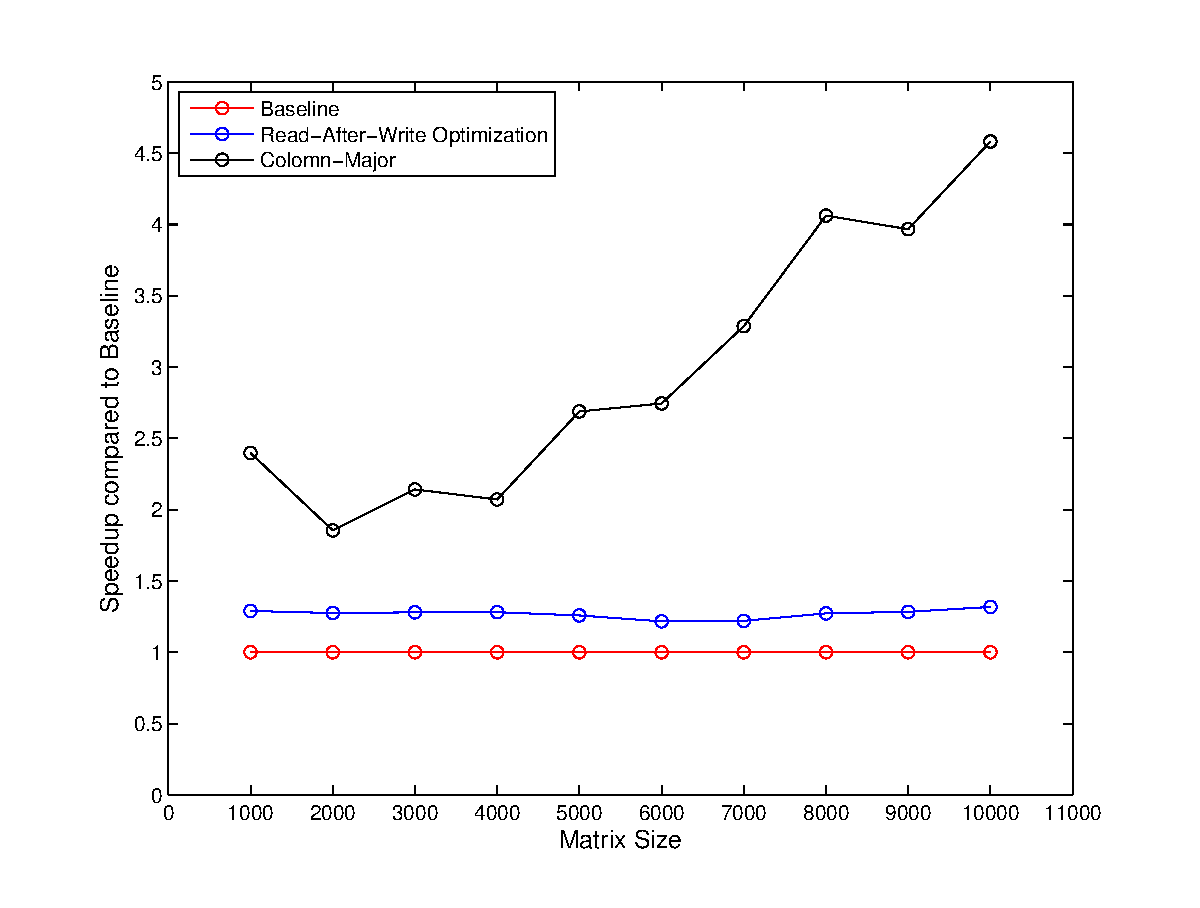
\includegraphics[width=0.5\textwidth]{vector_kernels}
%%\caption{Transactions on Singular Vector Design}
%%\label{fig:vector_kernels}
%%\end{figure}
%Read transactions are about twice of the write transactions on the global memory.
%Further analysis reveals that about 50\% of global memory transfers are read-after-write.
%Since it is a waste of time to read from global memory after writing to global memory,
%we improve the memory access performance by copying these values into the local memory and shared memory of the GPU.
%The global read transactions are reduced by 50\% compared to the baseline, while the write transactions remain the same, as shown as ``read/write optimization'' in Figure \ref{fig:transaction}. The speedup reaches to 1.2X compared to the baseline.
%To further optimize the access to the global memory,
%we change the matrix arrangement from row-major to column-major in the global memory. 
%As a result, the global load/store transactions are reduced by 50\%/25\% compared to ``read/write optimization'', respectively. 
%This is because column-major matrix have coalesced global memory accesses, which saves hundreds of transactions per thread. The speedup rises up to 4.5X compared to the baseline.

\subsection{Solution to Huge Matrices}
\label{sec_huge}
In our design, the maximum number of singular values can be processed on a singular GPU is $m_b = subinterval\_size \times thread\_block\_size$,
while the maximum number of singular vectors are determined by Equation (\ref{eq:max_size}).
\begin{equation}
m_t = \sqrt{U / (5 * S)}
\label{eq:max_size}
\end{equation}
where $U$ is the memory size of GPU, $5$ is the number of arrays required for a pair of singular vectors.
Usually, $m_b$ is much larger than $m_t$.
For Tesla K40c with 16GB memory, $m_t = 24K$, while $m_b = 262K$.
However, when the matrix size is larger than $m_t$, even larger than $m_b$,
the GPU kernels cannot obtain all singular values and vectors any more with a single GPU.
Therefore we derive a divide-and-conquer architecture to solve the huge matrix size as explained in this section.

When the size of a matrix is less than $m_b$ but larger than $m_t$,
we only need to divide the singular vectors into small sets, each of which can be processed by a single GPU.
However, if the matrix size is larger than $m_b$, we should divide both singular values and singular vectors into smaller partitions.
The singular value computations can be partitioned using $m_b$ directly, i.e., there are $l_b = \lfloor(n/m_b)\rfloor + 1$ partitions, each of which has $\lfloor(n/l_b)\rfloor$ singular values.

The division of singular vectors should take memory size into consideration.
The maximum number of partitions $l_t$ can be derived from Equation~(\ref{eq:max_length}) as follows:
\begin{equation}
l_t = \sqrt{U/(5 * n * 4)}
\label{eq:max_length}
\end{equation}
where $n$ is matrix size.
Thus, there should be $\lfloor(n/l_t)\rfloor+1$ partitions with
$\lfloor(n/l_t)\rfloor$ singular vectors in each partition.

% \subsubsection{Single GPU}
% For a single GPU, the execution between every pieces is serial {\bf FIXME: need discussion}.
% When one piece is finished, the GPU processes the next one, until the last one.
% Thus, the execution time is the summation of every data segment.
% Equation \ref{eq:max_length} also provides the theorical maximum matrix size can be processed on GPUs when set $l=1$.
% For Tesla K40c, the theorical maximum matrix size is $600$ million.
% However, only one thread works on GPU, if $l=1$.
% The singular vector kernel will not have any speedup compared to execution on CPU. {\bf FIXME this seems to be a big drawback of the design. We have to address this}

\subsection{Multiple GPUs on a server}
\label{sec_mgpu}
We implement the multiple-GPU version with Pthread libraries on one server
to control data partition and assignment to GPUs.
Pthreads is a nature choice for controlling multiple GPUs on a single server
because it uses shared memory architecture, dramatically reducing overheads
on data sharing. We also design an extensible interface between CPU and GPU,
 which is easy to scale to physical distributed GPUs, compared to CUDA asynchronization interface. In our design, each thread takes control of one GPU.

%According to the computing capacity of GPU, we separate the whole interval into several subintervals with different singular values in them.
%Each GPU processes its corresponding subintervals to obtain singular values and vectors.
%\textcolor{red}{Is this correct? is it "Each thread processes its corresponding subinterval to obtain singular values and vectors."?}

When matrix size becomes huge, the load balancing among multiple GPUs will be a problem for performance as shown in column 2 of Table \ref{tab:hugeResultTesla}.
To conquer this issue we also introduce a dynamic load-balancing method for a better speedup, where a GPU will take new tasks on unfinished subintervals as soon as it finishes its prior task.
%In this method, the whole intervals are divided into small pieces which can be processed in one GPU.
%when one GPU finishes its tasks and other GPU, it will check the tasks of other GPUs.

%\textbf{algorithm graph}
%For each subinterval, there are four global state : FREE, READY, BUSY, DONE.
%FREE means that the singular values in the subinterval have not been calculated yet.
%READY represents that singular value is ready to wait for further processing singular vector.
%BUSY is in the precessing of singular vectors.
%DONE means the singular vectors are ready in the subintervals.
%When singular values are READY, GPU will continue to calculate the singular vectors and set the state to BUSY.


%We also build a two-computer network to speed up the SVD.
%In our design, each computer has one GPU and communicated through sockets.



\vspace{-0.1in}
\section{Experimental Results} \label{sec:results}
\vspace{-0.1in}
In this section, we evaluate the performance of our bisection and twisted algorithm and compare it with prior SVD implementations on CPUs and GPUs.
%We also evaluate the performance of BT on huge matrices of size more than $100K$. 
%To our knowledge, this has not been done in any of the prior work so far. 
We implement the proposed BT algorithm on Tesla K40c with Kerpler architecture. 
Our implementation can run on GeForce 750Ti with Maxwell architecture and Quandro with Fermi architecture. 
%three different GPUs: GeForce 750 Ti, Quadro 600 and Tesla K40c,
%which differ in architecture, memory size and bandwidth listed in Table \ref{tab:spec}. 
In our implementations, we set the number of threads per GPU block as 512, which brings the better performance than other possible block sizes.
For the multi-GPU version of BT, we use 2 Tesla K40c that reside in the same server to scale up the size of matrices. 
%For the multi-GPU version of BT, we use a mixture of these GPUs that reside in the same server to scale up the size of matrices. 
%It is worth noting that our multi-GPU version of BT algorithm can be extended to physically distributed GPUs, i.e., GPUs on different hosts connected via a high speed network. 
%This part is however beyond the scope of this paper. 
%\begin{table}[h]
%\vspace{-0.2in}
%\caption{Specifications of Different GPUs}
%\vspace{-0.1in}
%\centering
%\begin{tabular}{|c|c|c|c|}
%\hline
%Specifications & GeForce 750 & Quandro 600 & Tesla K40 \\ \hline
%Architecture   &     Maxwell &       Fermi &    Kepler \\ \hline
%CUDA Cores     &         640 &          96 &      2880 \\ \hline
%TFLOPS         &       1.306 &       0.246 &      4.29 \\ \hline
%GPU Clock      &    1268 MHz &    1280 MHz &   745 MHz \\ \hline
%Mem Size       &        2 GB &        1 GB &     12 GB \\ \hline
%Mem Bandwidth  &   86.4 GB/s &   25.6 GB/s &  288 GB/s \\ \hline
%\end{tabular}
%\label{tab:spec}
%\vspace{-0.5in}
%\end{table}

\subsection{Comparison to Existing SVD Implementations}
We generate random bidiagonal matrices with double precision numbers in the range between 0 and 1.
In order to achieve high confidence on the results, we generate 10 random matrices, and for each matrix, our SVD algorithm is executed 10 times on a GPU (or two GPUs).
The standard deviation of their execution time is very small, so we report the average execution time across the 100 runs as the performance results.

We compare our algorithm with CULA GPU library \cite{cula}, Intel MKL library \cite{mkl}, Sheetal's QR implementation on S1070 \cite{09IPDPSQR}, and Liu's DC implementation on M2070 \cite{13CFDC}.
We measure the performance of CULA on Tesla K40c, and that of Intel MKL on an 8-core 2.53GHz CPU.
Until now, CULA library only has a QR based routine called culaDbdsqr.
Intel MKL library has both DC routine DBDSDC and QR routine DBDSQR. We select a faster routine DBDSDC for a comparison.
For Sheetal's \cite{09IPDPSQR} and Liu's \cite{13CFDC} implementation, we use the experimental results presendted in their paper. 

\begin{figure}[hbpt]
\vspace{-0.3in}
\centering
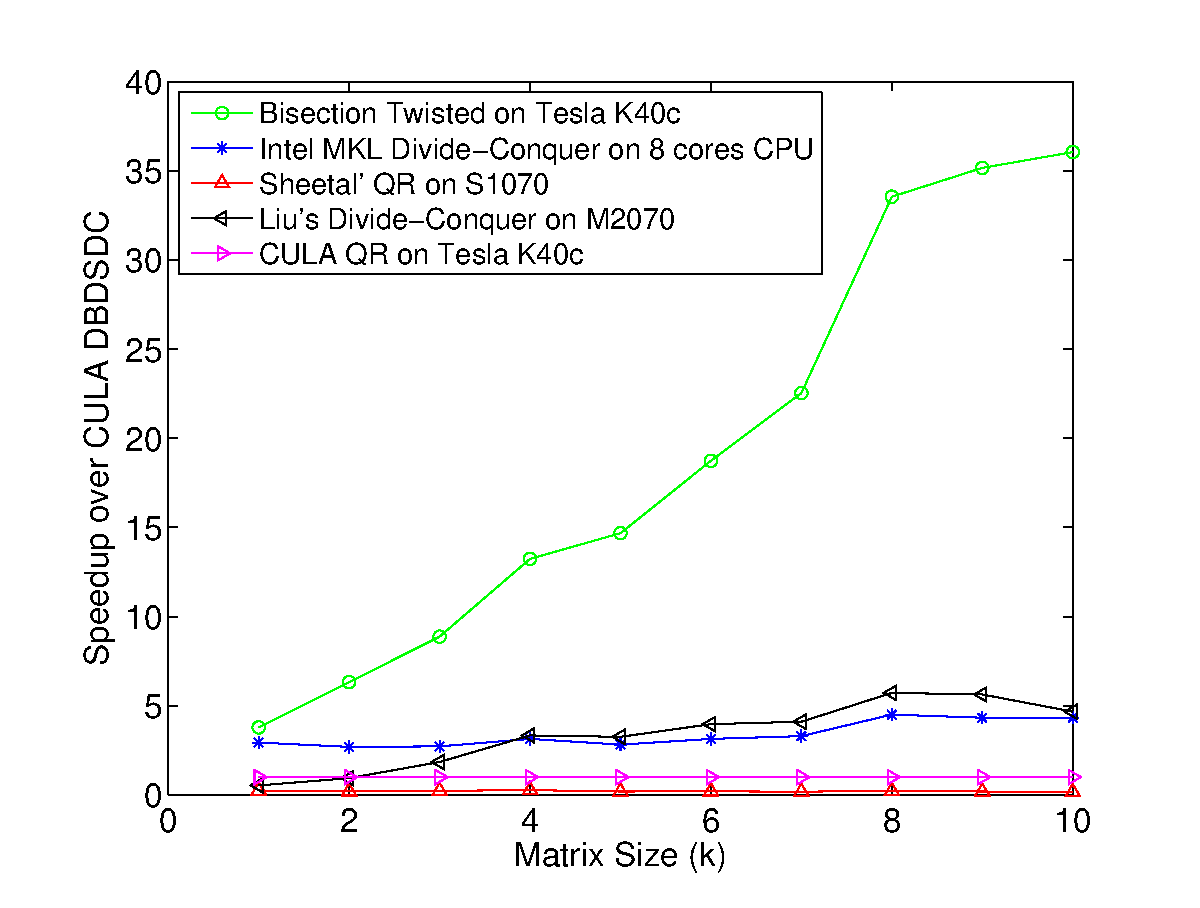
\includegraphics[width=0.5\textwidth,height=1in]{svd_speedup}
\vspace{-0.2in}
\caption{Overall Performance Comparison}
\label{fig:svd_speedup}
\vspace{-0.3in}
\end{figure}
Figure \ref{fig:svd_speedup} shows the performance comparison of BT
implementation on Tesla K40c GPU to other existing libraries
and implementations.
The x-axis is the size of input matrix, and the y-axis is the speedup
using CULA QR routine DBDSQR as the baseline.
Our BT algorithm achieves a speedup of 3.8 to 36 over CULA culaDbdsqr routine,
while Intel MKL DBDSDC routine has a 2.9 to 4.3 speedup on a 8 core CPU and Liu's implementation achieves only 0.5 to 4.7 speedup over CULA library.
On the other hand, Sheetal's implementation is about 3 to 5.3 times slower than CULA library.

The performance of BT scales well when the matrix size becomes large.
Overall, we achieve a speedup of 1.3 to 8.3 over the Intel MKL
DC implementation on CPU, 4 to 7.2 over the Liu's
DC method on GPU, and 15 to 288 over the QR implementation in the work by Sheetal et al.
Now let us take a look at each of the algorithms from the perspective of matrix size, Sheetal's QR implementation and Liu's DC implementation do not work at all when the dimensions of matrices are larger than 14K by 14K on their GPU with memory size of 16GB and 6GB, respectively. In contrast, in our implementation, the matrix size could reach 1 million by 1 million as shown in Table \ref{tab:hugeResultTesla}.

\if 0
\vspace{-0.2in}
\subsection{Performance Comparison on Different GPUs}

\subsubsection{Singular Value Computation}
\begin{figure}[hbpt]
\vspace{-0.3in}
\centering
  \subfigure[Execution time]
  {
    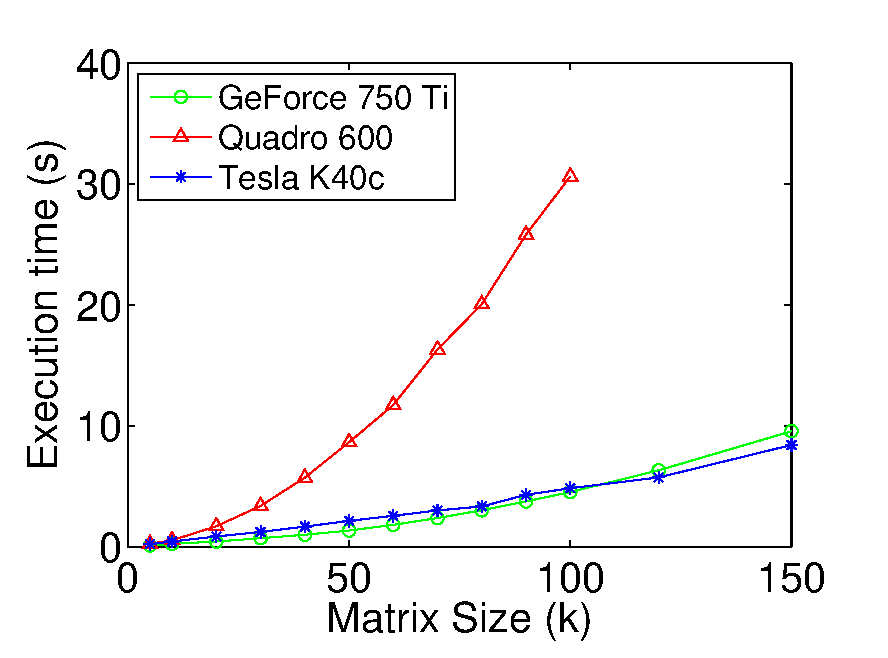
\includegraphics[width=0.3\textwidth,height=1in]{svd_val_gpus}
    \label{fig:svd_val}
  }
  \subfigure[Profiling Data]
  {
    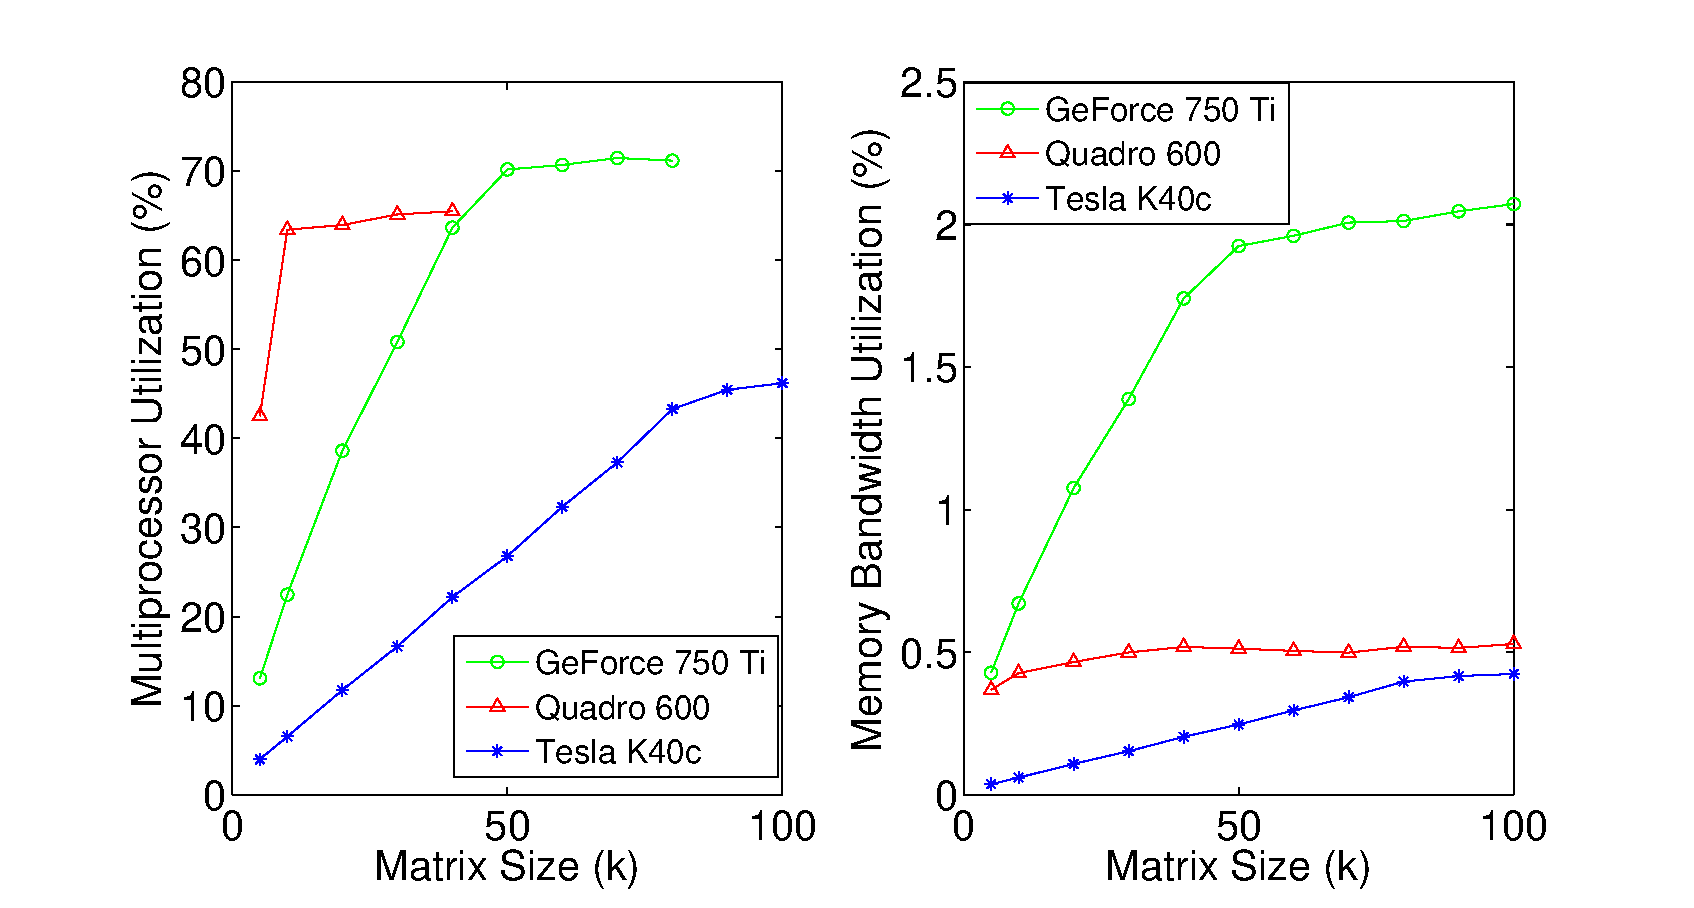
\includegraphics[width=0.6\textwidth,height=1in]{svd_val_gpus_prof}
    \label{fig:svd_val_prof}
  }
\vspace{-0.1in}
  \caption{Singular Value Kernel on Different GPUs}
  \label{fig:svdval}
\vspace{-0.3in}
\end{figure}

Figure \ref{fig:svd_val} shows the execution time of calculating singular values with our ``equal number division'' design on different GPUs with single-precision floating point.
Quadro has the worst performance, while performance of GeForce and Tesla are close to each other.
In particular, When the matrix size is less than $100K$, GeForce is slightly better. Otherwise, Tesla is better. 

To understand the reasons
of such performance differences, we conduct a series of profiling experiments.
Figure \ref{fig:svd_val_prof} shows the thread activity and memory bandwidth utilizations of singular value kernels on different GPUs, for matrices of size up to 
100K (unfortunately we are unable to get profiling data for matrices of larger size due to the overflow of profiling counters). 
The figure shows that the thread utilization reaches 70\% on Quadro and GeForce, and 50\% on Tesla. 
But the memory bandwidth utilization is only 0.1\%-2\%.
The main reason is that singular value computations rely on the fast shared memory
of GPUs due to its low memory requirements. That is, finding the singular
values is rather CPU-bound than memory-bound. 
As a result, the performance is determined largely by the number of CUDA cores and the ratio of thread activity on a GPU.

\subsubsection{Singular Vector Computation}
Figure \ref{fig:svd_vec} shows the execution time of singular vector kernel on different GPUs. 
It is easily seen that GeForce is about 8 times faster than
Quadro. This is because GeForce has a much higher memory bandwidth
than Quadro.
In addition, the device memory read/write transactions of GeForce are only 1/6 and 1/4 of those of Quadro, respectively.
The performance on Tesla is slightly better than that on GeForce.
Tesla has nearly the same device memory read transactions as GeForce does, while 3 times more write transactions than GeForce.
Yet Tesla is still the winner of the three because of its extremely high
bandwidth as listed in Table~\ref{tab:spec}.

\begin{figure}[hbpt]
\vspace{-0.3in}
\centering
  \subfigure[Execution time]
  {
    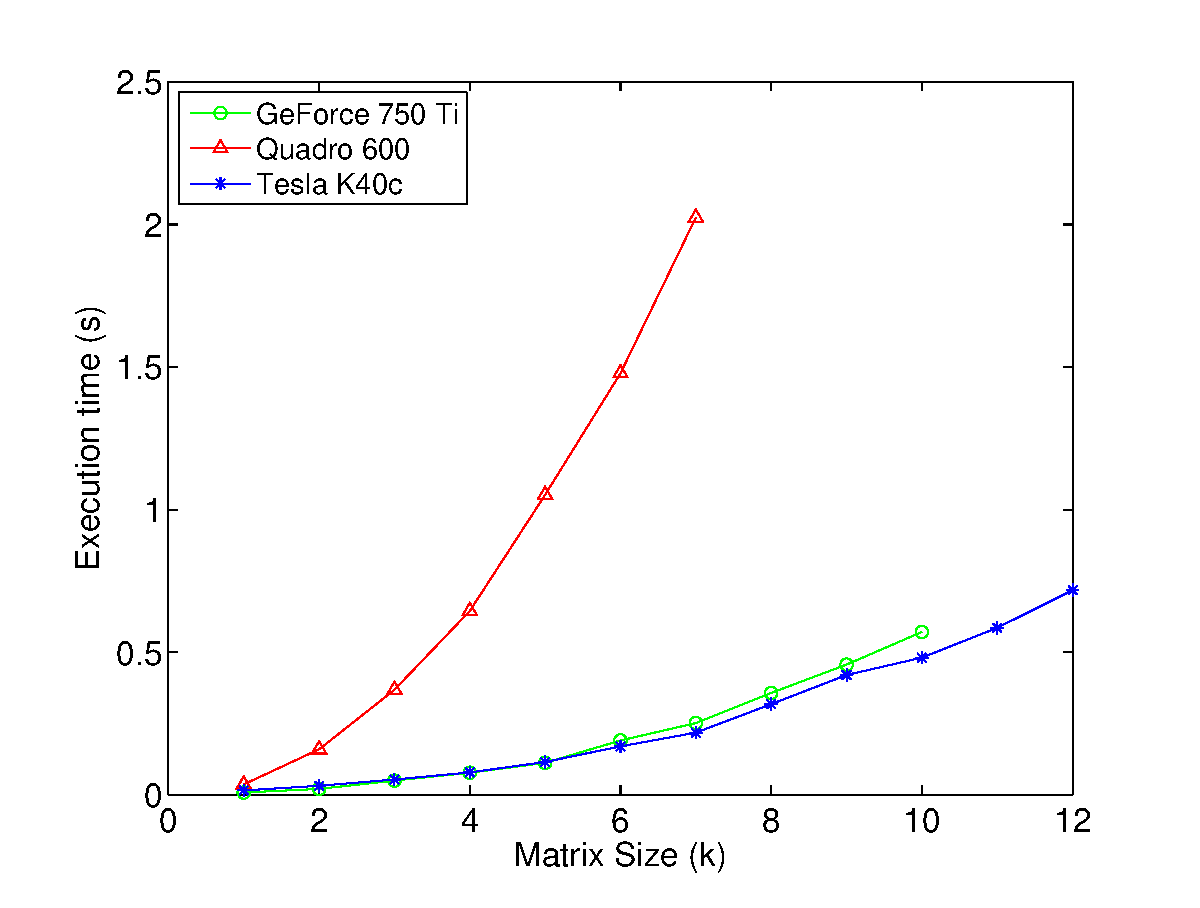
\includegraphics[width=0.3\textwidth,height=1in]{svd_vec_gpus}
    \label{fig:svd_vec}
  }
  \subfigure[Profiling Data]
  {
    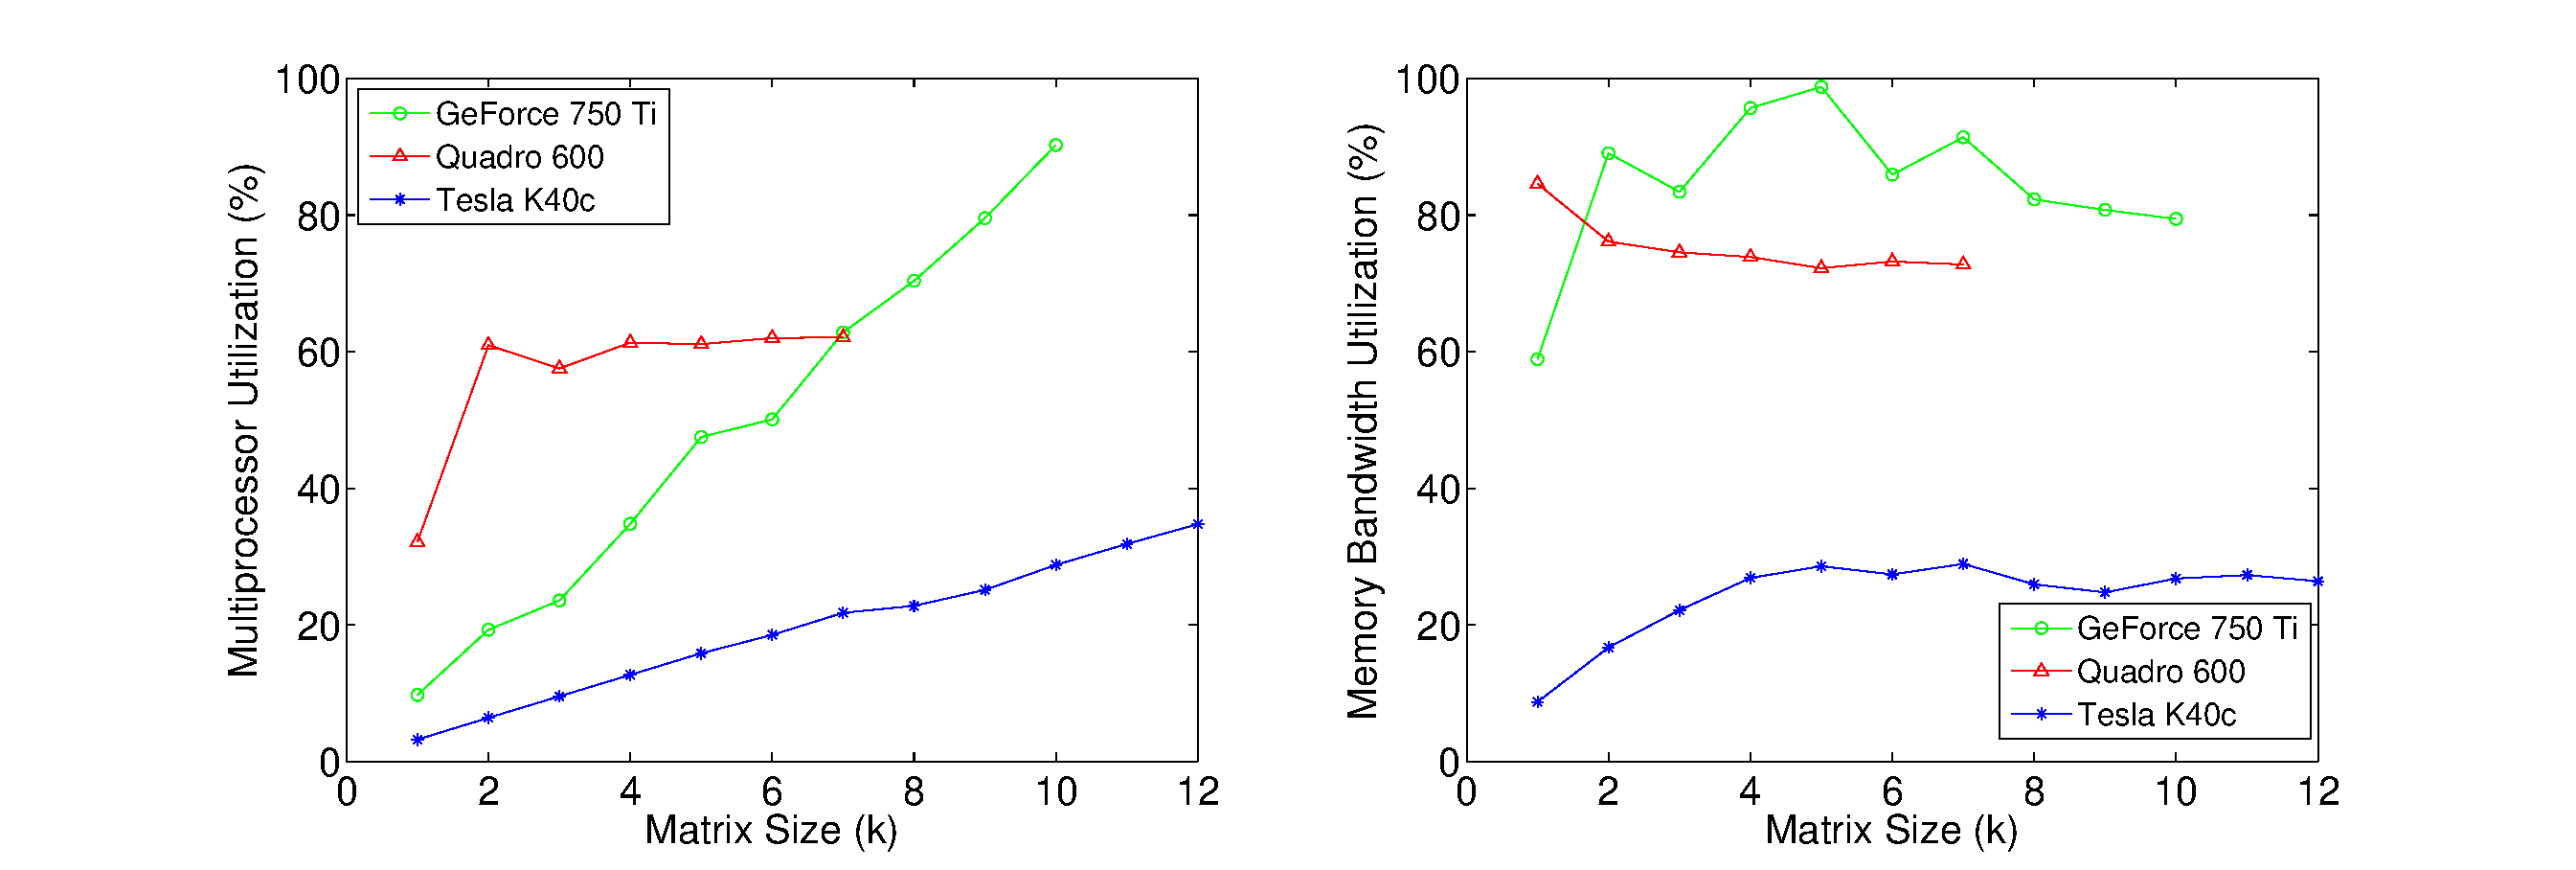
\includegraphics[width=0.6\textwidth,height=1in]{svd_vec_gpus_prof}
    \label{fig:svd_vec_prof}
  }
\vspace{-0.1in}
  \caption{Singular Vector Kernel on Different GPUs}
  \label{fig:svdvec}
\vspace{-0.3in}
\end{figure}

Figure \ref{fig:svd_vec_prof} shows thread and memory bandwidth utilizations of singular vector design on different GPUs. 
We can see from the figure that Quadro and GeForce reach a high memory utilization (80\%-99\%), while the memory utilization of Tesla is around 30\%. 
We also observe that when the matrix size is larger than 2K, the thread utilization keeps stable on Quadro. 
This is because the ratio of stall caused by memory is 70\%, implying that there are a lot of threads waiting on data transfer.
\fi 

\subsection{Huge Size Result}
Table \ref{tab:hugeResultTesla} shows the performance of huge size matrix with double-precision floating-point numbers on a single Tesla and two Tesla GPUs on a server. For two Telsa GPUs, we compared static workload allocation (50\%/50\%) and dynamic allocation where each GPU is tracked constantly by the host CPU and assigned new workload as soon as it finishes the current kernel. 
When matrix size reaches 1 million by 1 million our BT algorithm reaches the results in 54801 seconds with a single Telsa, and 35607 seconds with two Telsa GPUs. This is a 1.54X speedup.
\begin{table}[h]
\vspace{-0.3in}
\caption{Performance of Huge Size Matrix with double floating-point on Tesla}
\vspace{-0.1in}
\centering
\begin{tabular}{|c|c|c|c|}
\hline
Matrix Size &  Tesla  & Static & Dynamic \\ \hline
% 10K*10K    &   1.5s  &  1.9s / 1.2s &  0.9s / 2.5s \\ \hline
% 20K*20K    &   7.9s  &  7.4s / 5.7s &  3.1s / 10s \\ \hline
% 30K*30K    &    25s  &   17s /  14s &  12s  / 19s \\ \hline
% 40K*40K    &    38s  &   27s /  24s &  26s / 26s \\ \hline
 50K*50K    &    71s  &   50s /  45s &  44s / 44s \\ \hline
% 80K*80K    &   180s  &  121s / 103s &  111s / 116s \\ \hline
 100K*100K  &   341s  &  217s / 189s &  210s / 202s \\ \hline
% 120K*120K  &   524s  &  326s / 286s &  311s / 311s \\ \hline
 150K*150K  &   864s  &  524s / 467s &  498s / 507s \\ \hline
% 180K*180K  &   966s  & 1207s / 532s &  602s / 607s \\ \hline
 200K*200K  &  1407s  &  955s / 827s &  849s / 858s \\ \hline
% 250K*250K  &  1949s  & 1286s / 1118s & 1199s / 1204s\\ \hline
 300K*300K  &  3490s  & 2234s / 1906s & 2123s / 2110s\\ \hline
 400K*400K  &  6559s  & 4110s / 3709s & 3853s / 3871s\\ \hline
 500K*500K  & 12282s  & 7371s / 6916s  & 7148s / 7129s\\ \hline
 800K*800K  & 40311s  & 22454s / 21627s &  22046s / 22026s   \\ \hline
 1000K*1000K & 54801s  & 36119s / 35071s   &  35587s / 35607s \\ \hline
\end{tabular}
\label{tab:hugeResultTesla}
\vspace{-0.2in}
\end{table}

\subsection{Profiling Analysis of GPU Kernels}

\subsubsection{Comparison of Two Different Singular Value Designs}
We compare the execution time on two different singular value kernels:
``equal length division'' versus ``equal number division''. Each
method has two phases: (1) divide the interval into subintervals and
(2) calculate singular values in each subinterval.
%For the length division design, we selects the minimal execution time corresponding to red point curve in figure \ref{fig:length_block_num}.
%For the number division design, we selects the minimal number of blocks that is able to allocated, since the execution time does not vary much between the minimal number of blocks and the optimal nubmer of blocks.
\begin{figure}[hbpt]
\vspace{-0.3in}
\centering
  \subfigure[Comparison of Equal Length Division and Equal Number Division. ``Interval Division in EL'' is negligible.]
  {
    \includegraphics[width=0.4\textwidth]{compare_value_kernel}
    \label{fig:compare_value_kernel}
  }
  \subfigure[Memory Transactions on Singular Vector Design]
  {
    \includegraphics[width=0.4\textwidth]{transaction}
    \label{fig:transaction}
  }
\vspace{-0.1in}
%  \caption{Orthogonality of Singular Vector}
%  \label{fig:ortho}
%\vspace{-0.3in}
\end{figure}
%\begin{figure}[hbpt]
%\centering
%\includegraphics[width=0.4\textwidth]{compare_value_kernel}
%\caption{Comparison of Equal Length Division and Equal Number Division. ``Interval Division in EL'' is negligible. }
%\label{fig:compare_value_kernel}
%\vspace{-0.10in}
%\end{figure}
Figure \ref{fig:compare_value_kernel} shows the detailed execution time breakdown for each phase of both methods (``Interval Division'' time for ``equal-length division'' is negligible) on Tesla K40c.
From the figure, we can see that when the matrix size is less than 9K, the equal length division version runs a little faster than equal number division version.
However, when the matrix size exceeds 9K, the execution time of the equal length division version increases dramatically, while the execution time of equal number division version still rises linearly.
And in this case, 
%even the time to divide the interval is noticeably large, the balanced number
%of singular values in a subinterval helps improving the overall performance.
even though the time to divide the interval is noticeably
large, the balanced number of singular values in a subinterval
still yields much better performance.
Thus, the equal number division version is obviously the winner when the matrix size becomes larger than 9K.

\subsubsection{Memory Access Optimization}
We evaluate the memory optimization techniques on improving the performance
of singular vector calculation. As depicted in Figure \ref{fig:transaction},
%\begin{figure}[hbpt]
%\centering
%\includegraphics[width=0.4\textwidth]{transaction}
%\caption{Memory Transactions on Singular Vector Design}
%\label{fig:transaction}
%\vspace{-0.15in}
%\end{figure}
in the baseline design,
Global memory Load Transactions (GLT) are about twice of the Global memory Store Transactions (GST) on the global memory.
As there are 50\% of global memory transfers are read-after-write, we improve the memory access performance by copying these values into the local memory and shared memory of the GPU. As a result, the GLT are reduced by 50\% compared to the baseline, while the GST remains the same, labeled as ``Read/Write Optimization'' in Figure \ref{fig:transaction}. The speedup on singular vector calculation reaches to 1.2X compared to the baseline.
Changing the matrix arrangement from row-major to column-major in the global memory 
reduces GLT and GST by 50\% and 25\%, respectively, compared to ``Read/Write optimization''. 
This is because column-major matrix have coalesced global memory accesses, which saves hundreds of transactions per thread. The speedup rises up to 4.5X compared to the baseline.

\subsection{Accuracy Analysis}
\subsection{Tolerance in Bisection Algorithm}
Since the bisection algorithm is an approximate algorithm to calculate the singular values, we should test the effect of different error tolerance.
The error tolerance $err$ means that the error between the singular values of our algorithm and the actual singular values are less than $err$.
It determines the accuracy of singular value and therefore the orthogonality of singular vectors.
As we know, the more accuracy of singular values are, the more execution time should be spent.
However, it is important to know the incremental execution time to determine which error tolerance is suitable for different applications.
We test our algorithm on different error tolerance.
The error tolerance is between $10^{-5}$ to $10^{-16}$ with tenfolder decreasing.

%\textbf{I'm still thinking how to draw this figure.}
\begin{figure}[hbpt]
\centering
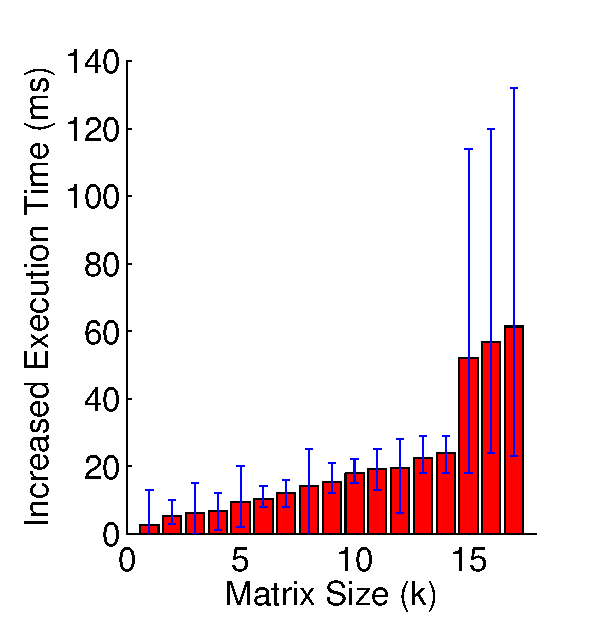
\includegraphics[width=0.5\textwidth]{tolerance}
\caption{Average Extra Execution Time When the accuracy increase Performance Comparision}
\label{fig:tolerance}
\end{figure}
Figure \ref{fig:tolerance} shows the average increased execution time when the accuracy of singular values goes up a higher level on different matrix size.
In other word, it shows the average increased execution time when the error tolerance becomes smaller from $10^{-x}$ to $10^{-(x+1)}$.
From the figure, we can see that when matrix size is smaller than 12000, the additional execution time is only less than $20 ms$ when the error tolerance rises a level.
When the matrix size is larger than 15000, the additional execution time is a little higher about $40 ms$ per level.

\subsubsection{Orthogonality of Singular Vector}
In this section, I will show the orthogonality of singular vectors. 
The multiplication of singular vectors is shown in \ref{fig:ortho_img}. The white diagonal are 1s, and the black are 0s. 
The error distribution of orthogonality is shown in \ref{fig:ortho_err}. Almost all the errors are close to 0.
\begin{figure}[hbpt]
\vspace{-0.3in}
\centering
  \subfigure[Orthogonal Error]
  {
    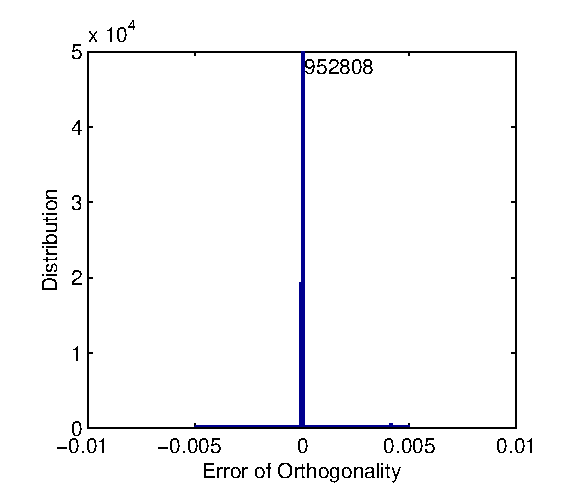
\includegraphics[width=0.4\textwidth]{ortho_err}
    \label{fig:ortho_err}
  }
  \subfigure[Image of Singular Vector Multiplication]
  {
    \includegraphics[width=0.4\textwidth]{orthogonal}
    \label{fig:ortho_img}
  }
\vspace{-0.1in}
  \caption{Orthogonality of Singular Vector}
  \label{fig:ortho}
\vspace{-0.3in}
\end{figure}


\section{Related Work}
\label{sec:related}
General purpose GPUs have become important processing engines for computationally intensive workloads due to their highly parallel computing architectures.
Linear algebra operations are among the first batch of libraries accelerated with GPUs.
There are various such accelerated libraries, i.e.,  CUBLAS, CULA, MAGMA. The BLAS (Basic Linear Algebra Subprograms) are routines supported by Nvidia \cite{cublas} that provide standard building blocks for performing basic vector and matrix operations. CUBLAS is an implementation of BLAS and provides many solutions for common linear algebra operations. 
However, it does not provide solutions to complex linear algebra problems, such as QR decomposition, LU decomposition and SVD.
CULA consists of commercial hybrid GPU accelerated linear algebra routines\cite{cula} that support high-level linear algebra operations.
Among them, the singular value decomposition employs QR algorithm, which is not an effective algorithm when the matrix size becomes significantly large.
MAGMA aims to achieve high performance and portability across a wide range of multi-core architectures and hybrid systems respectively\cite{magma}.

QR, the most commonly used algorithm for computing singular values and vectors, 
is regarded as a powerful and effective algorithm with high accuracy
and numerical stability\cite{97bookalgebra}. 
Their implementation shows a speedup of up to 8 over the Intel MKL QR implementation \cite{mkl}.
The first SVD algorithm with CUDA programming is implemented by Sheetal et al.\cite{09IPDPSQR}. With parallelized QR iteration algorithm using CUBLAS library on GPU, they achieved a speedup of up to 8 over the Intel MKL QR implementation.
However, the QR-iteration algorithm has its drawback on parallelization due to its heavy data dependency.
The algorithm requires $O(n^3)$ to complete the diagonalization and its decomposition time is intolerable as size of matrices increase.
%Moreover, calling too much CUBLAS kernels also reduces the performance in the GPU design.

Liu et al. use a divide-and-conquer approach to solve SVD on a heterogeneous CPU-GPU system \cite{13CFDC}.
It is almost 7 times faster than CULA QR algorithm executing on the same device M2070, and up to 33 times faster than LAPACK.
However, DC approach is relatively inaccurate during the merging phase, especially when the data scale is huge.
In the worst case, it will require $O(n^3)$ to complete SVD, if the singular values are in a dense distribution\cite{97bookalgebra}.
%This is because the implementation that makes use of pipeline architecture in a heterogeneous architecture does not make full use of resources on GPUs and the frequent data transfer between GPU and CPU dramatically slow down the execution time.

Vedran\cite{14arxivjacobi} presents a hierarchically blocked one-sided Jacobi algorithm for the singular value decomposition on both single and multiple GPU architectures. 
The algorithm maintains high accuracy in singular values and vectors. Due to the speed limitation of the algorithm, even with full optimizations and a high speedup compared to the same algorithm on CPU, the execution time is still more than that of Sheetal's QR implementation.


In \cite{99clustering} Drineas et al. provide a clustered SVD algorithm for large matrices. The algorithm divides a set of $n$ points into $k$ clusters, where $k$ is much less than $n$ on CPU.
It is an approximation algorithm to obtain only one subset of singular values
and vectors. Our BT algorithm can compute the complete SVD, thus is not
directly compared with \cite{99clustering}. 
%They experimentally
%evaluate the accuracy and speed of this algorithm for image matrices, using
%various probability distributions to perform the sampling\cite{01randomizedSVD,01mentoSVD}.



\input{6_conclusion}

\section*{Acknowledgment}
This work is support in part by the National Science Foundation under grant number ACI-1440737. 

\vspace{-0.1in}
\bibliographystyle{splncs}
\bibliography{ref}

\end{document}
